\documentclass[11pt,a4paper]{article}
\usepackage[margin=2.5cm]{geometry}
\usepackage{amsmath,amssymb,amsthm}
\usepackage{braket}
\usepackage{physics}
\usepackage{hyperref}
\usepackage{xcolor}
\usepackage{booktabs}
\usepackage{algorithm}
\usepackage{algpseudocode}
\usepackage{tikz}
\usetikzlibrary{arrows.meta, positioning, shapes}

\title{\textbf{Quantum State Preparation via Latent-Space Reinforcement Learning}\\
\large A Physics-Informed World Model for Noisy Quantum Devices}
\author{Quantum Gym Project}
\date{April 2026}

\newtheorem{definition}{Definition}
\newtheorem{remark}{Remark}

\begin{document}
\maketitle
\tableofcontents
\newpage

% ============================================================
\section{Problem Formulation}
% ============================================================

\subsection{Quantum State and Target}

We work with an $n=3$ qubit system. The Hilbert space is
\begin{equation}
    \mathcal{H} = \left(\mathbb{C}^2\right)^{\otimes 3}, \quad \dim \mathcal{H} = 8.
\end{equation}

The target state is the Greenberger--Horne--Zeilinger (GHZ) state:
\begin{equation}
    \ket{\text{GHZ}} = \frac{\ket{000} + \ket{111}}{\sqrt{2}}.
\end{equation}

Starting from the computational zero state $\ket{\psi_0} = \ket{000}$, the goal is to
find a parameterised circuit $U(\boldsymbol{\theta})$ such that
\begin{equation}
    F\bigl(U(\boldsymbol{\theta})\ket{000},\, \ket{\text{GHZ}}\bigr)
    = \left|\bra{\text{GHZ}} U(\boldsymbol{\theta}) \ket{000}\right|^2 \geq 1 - \varepsilon.
\end{equation}

\subsection{Fubini--Study Metric}

The natural distance on the space of pure quantum states (the projective Hilbert space
$\mathbb{CP}^{2^n-1}$) is the \emph{Fubini--Study metric}:
\begin{equation}
    d_{\mathrm{FS}}(\ket{\psi}, \ket{\phi})
    = \arccos\!\left|\braket{\psi}{\phi}\right|
    \in \left[0, \frac{\pi}{2}\right].
\end{equation}

We use the closely related \emph{trace distance} as a scalar score:
\begin{equation}
    D(\psi, \phi) = \frac{1}{2}\|\rho_\psi - \rho_\phi\|_1
    = \sqrt{1 - \left|\braket{\psi}{\phi}\right|^2}
    = \sin\bigl(d_{\mathrm{FS}}(\ket{\psi},\ket{\phi})\bigr),
\end{equation}
where $\rho_\psi = \ket{\psi}\bra{\psi}$.

\subsection{Key Requirement: Smooth Manifold}

For the reinforcement learning agent to generalise, small angle increments must correspond
to small displacements in $\mathcal{H}$. Given a layer parameterised by $\boldsymbol{\alpha}$
and perturbed by $\delta\boldsymbol{\alpha}$:
\begin{equation}
    d_{\mathrm{FS}}\!\bigl(U(\boldsymbol{\alpha})\ket{\psi},\,
    U(\boldsymbol{\alpha}+\delta\boldsymbol{\alpha})\ket{\psi}\bigr)
    \;\propto\; \|\delta\boldsymbol{\alpha}\|
    \quad\text{for }\|\delta\boldsymbol{\alpha}\| \ll 1.
\end{equation}
This is the motivating constraint for the ansatz design in Section~\ref{sec:ansatz}.

% ============================================================
\section{Ansatz Design}\label{sec:ansatz}
% ============================================================

\subsection{Layer Structure}

Each layer $r$ of the forward ansatz applies:
\begin{equation}
    L_r(\boldsymbol{\theta}_r) =
    \mathrm{CR}(\alpha_{12}^{(r)}, 1{\to}2)\;
    \mathrm{CR}(\alpha_{01}^{(r)}, 0{\to}1)\;
    \bigotimes_{q=0}^{2} R_y(\theta_q^{(r)}),
\end{equation}
where the parameter vector per layer is
\begin{equation}
    \boldsymbol{\theta}_r = \bigl[\theta_0^{(r)},\, \theta_1^{(r)},\, \theta_2^{(r)},\,
    \alpha_{01}^{(r)},\, \alpha_{12}^{(r)}\bigr] \in \mathbb{R}^5.
\end{equation}

\subsubsection*{Single-qubit gate}
\begin{equation}
    R_y(\theta) = e^{-i\frac{\theta}{2}Y} =
    \begin{pmatrix} \cos\frac{\theta}{2} & -\sin\frac{\theta}{2} \\
    \sin\frac{\theta}{2} & \cos\frac{\theta}{2} \end{pmatrix}.
\end{equation}

\subsubsection*{Controlled-$R_y$ (CR) gate}
\begin{equation}
    \mathrm{CR}(\alpha) = \ket{0}\bra{0} \otimes I + \ket{1}\bra{1} \otimes R_y(\alpha)
    =
    \begin{pmatrix} 1 & 0 & 0 & 0 \\
    0 & 1 & 0 & 0 \\
    0 & 0 & \cos\frac{\alpha}{2} & -\sin\frac{\alpha}{2} \\
    0 & 0 & \sin\frac{\alpha}{2} & \cos\frac{\alpha}{2}
    \end{pmatrix}.
\end{equation}

For $\alpha \to 0$, $\mathrm{CR}(\alpha) \to I \otimes I$ continuously, ensuring smooth
Hilbert-space displacements. The inverse is simply $\mathrm{CR}(-\alpha)$.

\subsection{Full Circuit}

The $N$-layer forward circuit from $\ket{000}$ is:
\begin{equation}
    \ket{\psi_N} = U_N(\boldsymbol{\Theta})\ket{000},
    \qquad
    U_N(\boldsymbol{\Theta}) = \prod_{r=1}^{N} L_r(\boldsymbol{\theta}_r),
\end{equation}
where $\boldsymbol{\Theta} = (\boldsymbol{\theta}_1, \ldots, \boldsymbol{\theta}_N) \in \mathbb{R}^{5N}$.

\subsection{Inverse Layer (Backward Pass)}

Since $R_y^{-1}(\theta) = R_y(-\theta)$ and $\mathrm{CR}^{-1}(\alpha) = \mathrm{CR}(-\alpha)$,
the exact inverse of $L_r$ is:
\begin{equation}
    L_r^{-1}(\boldsymbol{\theta}_r) =
    \bigotimes_{q=0}^{2} R_y(-\theta_q^{(r)})\;
    \mathrm{CR}(-\alpha_{01}^{(r)}, 0{\to}1)\;
    \mathrm{CR}(-\alpha_{12}^{(r)}, 1{\to}2).
\end{equation}

\subsection{Hardware Quantization}

The device (Quantum Inspire, Zebra/Tuna-17) quantizes angles to multiples of $\pi/36$ ($5°$).
Let $\Delta_{\mathrm{device}} = \pi/36$. For the beam search we use a coarser step
$\Delta_{\mathrm{search}} = \pi/18$ (two device steps), chosen so that
\begin{equation}
    \frac{\pi}{2} = 9 \times \frac{\pi}{18} = 9\,\Delta_{\mathrm{search}},
\end{equation}
meaning the optimal GHZ rotation angle is exactly reachable on the discrete grid.

% ============================================================
\section{Step 1: Beam Search in Simulation}\label{sec:beamsearch}
% ============================================================

\subsection{Forward Search Objective}

We want circuits that achieve high GHZ fidelity while keeping trajectories smooth.
The beam search maximises:
\begin{equation}
    \mathcal{F}(\boldsymbol{\Theta}) = F\bigl(\ket{\psi_N}, \ket{\text{GHZ}}\bigr)
    = \left|\bra{\text{GHZ}} U_N(\boldsymbol{\Theta})\ket{000}\right|^2.
\end{equation}

\subsection{Discrete Action Space}

At each round $r$, the search perturbs the previous angles by:
\begin{equation}
    \boldsymbol{\theta}_r = \boldsymbol{\theta}_{r-1} + \Delta\boldsymbol{\theta}_r,
    \qquad
    \Delta\boldsymbol{\theta}_r \in \{-\Delta_{\mathrm{search}},\, 0,\, +\Delta_{\mathrm{search}}\}^5.
\end{equation}
This gives $3^5 = 243$ possible actions per step.

\subsection{Beam Search Algorithm}

\begin{algorithm}
\caption{Forward Beam Search for GHZ Preparation}
\begin{algorithmic}[1]
\State Initialise $W$ beams with random $\boldsymbol{\theta}_1 \sim \mathcal{U}(-\Delta, \Delta)^5$
\For{$r = 1, \ldots, N_{\max}$}
    \For{each beam $b$ with state $\ket{\psi_r^{(b)}}$}
        \For{each action $\Delta\boldsymbol{\theta} \in \{-\Delta, 0, \Delta\}^5$}
            \State $\boldsymbol{\theta}' \leftarrow \boldsymbol{\theta}_r^{(b)} + \Delta\boldsymbol{\theta}$
            \State $\ket{\psi'} \leftarrow L(\boldsymbol{\theta}')\ket{\psi_r^{(b)}}$
            \State Score: $\mathcal{F}' \leftarrow |\braket{\mathrm{GHZ}}{\psi'}|^2$
        \EndFor
    \EndFor
    \State Keep top-$W$ candidates (80\% greedy + 20\% random exploration)
    \If{$\max_b \mathcal{F}_r^{(b)} \geq 0.999$} \textbf{break} \EndIf
\EndFor
\State \Return trajectories sorted by $\mathcal{F}$ descending
\end{algorithmic}
\end{algorithm}

% ============================================================
\section{Step 2: Local Refinement}\label{sec:refinement}
% ============================================================

The discrete beam search is limited by the grid resolution $\Delta_{\mathrm{search}}$.
Starting from the best beam trajectory $\boldsymbol{\Theta}^*$, we refine with
continuous optimisation:
\begin{equation}
    \boldsymbol{\Theta}^{**} = \arg\min_{\boldsymbol{\Theta}}
    \;\Bigl[-\mathcal{F}(\boldsymbol{\Theta})\Bigr]
    = \arg\min_{\boldsymbol{\Theta}}
    \;\Bigl[1 - \left|\bra{\text{GHZ}} U_N(\boldsymbol{\Theta})\ket{000}\right|^2\Bigr],
\end{equation}
using L-BFGS-B with gradient computed via statevector simulation.
This pushes $\mathcal{F}: 87\% \to 99\%+$.

After optimisation, the angles are re-quantized for hardware:
\begin{equation}
    \tilde{\theta} = \Delta_{\mathrm{device}}\cdot \mathrm{round}\!\left(\frac{\theta^{**}}{\Delta_{\mathrm{device}}}\right).
\end{equation}

% ============================================================
\section{Step 3: Shadow Fingerprinting and QI Acquisition}\label{sec:shadow}
% ============================================================

\subsection{Classical Shadow Fingerprint}

To encode a quantum state $\ket{\psi}$ into a fixed-dimensional feature vector, we use
\emph{classical shadow tomography}. For $n=3$ qubits, a shadow of size $K$ gives an
unbiased estimator for all $k$-local Pauli observables ($k \leq 3$).

The fingerprint $\mathbf{x}(\psi) \in \mathbb{R}^{63}$ contains expectation values of:
\begin{itemize}
    \item 1-local Paulis: $\{X_i, Y_i, Z_i\}$ for $i \in \{0,1,2\}$ — 9 values
    \item 2-local Paulis: $\{P_i P_j\}$ for $i < j$, $P \in \{X,Y,Z\}$ — 27 values
    \item 3-local Paulis: $\{P_0 P_1 P_2\}$ — 27 values
\end{itemize}
Total: $9 + 27 + 27 = 63$ features.

Each estimator from $K$ shots satisfies:
\begin{equation}
    \hat{o}_P = \mathbb{E}_{\text{shadow}}\!\left[\mathrm{tr}(P\,\hat{\rho})\right]
    = \mathrm{tr}(P\,\rho_\psi), \qquad
    \mathrm{Var}[\hat{o}_P] = \mathcal{O}(K^{-1}).
\end{equation}

\subsection{Budget-Aware QI Circuit Selection}

Running circuits on QI is expensive (queue time). We select $M \approx 50$ circuits
maximising information gain subject to a budget:
\begin{equation}
    \max_{\mathcal{S} \subseteq \mathcal{C},\, |\mathcal{S}| \leq M}
    \;\mathrm{InfoGain}(\mathcal{S}),
\end{equation}
where the selected set $\mathcal{S}$ is constructed greedily:

\medskip
\textbf{Priority 1 — Anchor points} ($\sim 10$ circuits):
\begin{equation}
    \mathcal{S}_1 = \bigl\{\ket{000},\; \ket{\mathrm{GHZ}},\;
    \ket{\psi_{r^*}} \text{ for } r^* \in \{1, 3, 5, 7, 9\}\bigr\}.
\end{equation}

\textbf{Priority 2 — Noise characterization} ($\sim 20$ circuits):
Single-gate benchmarks $\{R_y(\theta)\ket{0}\}_\theta$ and
$\{\mathrm{CR}(\alpha)\ket{10}\}_\alpha$ to fit a noise model.

\textbf{Priority 3 — Trajectory diversity} ($\sim 20$ circuits):
Sparse steps from the top-3 beam trajectories.

% ============================================================
\section{Step 4: Variational Autoencoder (VAE)}\label{sec:vae}
% ============================================================

\subsection{Architecture}

The VAE encodes shadow fingerprints $\mathbf{x} \in \mathbb{R}^{63}$ to a
low-dimensional latent space $\mathbf{z} \in \mathbb{R}^d$ ($d=2$ for visualization).

The encoder outputs a Gaussian posterior:
\begin{equation}
    q_\phi(\mathbf{z} | \mathbf{x}) = \mathcal{N}\!\left(\boldsymbol{\mu}_\phi(\mathbf{x}),\;
    \mathrm{diag}\!\left(e^{\boldsymbol{\sigma}^2_\phi(\mathbf{x})}\right)\right).
\end{equation}

The decoder reconstructs the fingerprint:
\begin{equation}
    p_\theta(\mathbf{x} | \mathbf{z}) = \mathcal{N}\!\left(\hat{\mathbf{x}}_\theta(\mathbf{z}),\,
    \sigma^2_{\mathrm{dec}} I\right).
\end{equation}

\subsection{Standard VAE Loss}

\begin{equation}
    \mathcal{L}_{\mathrm{VAE}}(\phi, \theta; \mathbf{x})
    = \underbrace{\mathbb{E}_{q_\phi}\!\left[\log p_\theta(\mathbf{x}|\mathbf{z})\right]}_{\text{reconstruction}}
    - \underbrace{\beta\, D_{\mathrm{KL}}\!\left[q_\phi(\mathbf{z}|\mathbf{x})\,\|\,p(\mathbf{z})\right]}_{\text{regularisation}},
\end{equation}
where $p(\mathbf{z}) = \mathcal{N}(0, I)$ is the prior and $\beta$ controls the
disentanglement--fidelity trade-off via KL annealing:
\begin{equation}
    \beta(e) = \beta_{\min} + \left(\beta_{\max} - \beta_{\min}\right)
    \cdot \min\!\left(1,\, \frac{e}{E_{\mathrm{warmup}}}\right).
\end{equation}

\subsection{Metric Loss (Physics-Informed)}

To ensure the latent geometry reflects the Fubini--Study metric, we add:
\begin{equation}
    \mathcal{L}_{\mathrm{metric}} =
    \sum_{(i,j) \in \mathcal{T}}
    \Bigl(\|\boldsymbol{\mu}_i - \boldsymbol{\mu}_j\|^2
    - \lambda\, d_{\mathrm{FS}}^2(\ket{\psi_i}, \ket{\psi_j})\Bigr)^2,
\end{equation}
where $\mathcal{T}$ is the set of consecutive transition pairs. This forces
nearby states in $\mathcal{H}$ to be nearby in the latent space.

\subsection{Sim-to-Real Fine-Tuning}

After training on simulation data, the encoder $\phi$ is fine-tuned on QI fingerprints
$\{\mathbf{x}_j^{\mathrm{QI}}\}$ with the decoder frozen ($\theta$ fixed):
\begin{equation}
    \phi^* = \arg\min_\phi
    \sum_j \mathcal{L}_{\mathrm{VAE}}(\phi, \theta_{\mathrm{frozen}};\, \mathbf{x}_j^{\mathrm{QI}}),
\end{equation}
using a small learning rate to preserve the latent geometry while aligning QI points correctly.

\subsection{Joint Training Objective}

The full training loss is:
\begin{equation}
    \mathcal{L}_{\mathrm{total}} =
    \mathcal{L}_{\mathrm{VAE}}
    + \lambda_1 \mathcal{L}_{\mathrm{transition}}
    + \lambda_2 \mathcal{L}_{\mathrm{metric}}
    + \lambda_3 \mathcal{L}_{\mathrm{noise}},
\end{equation}
with $\mathcal{L}_{\mathrm{transition}}$ defined in Section~\ref{sec:worldmodel}.

% ============================================================
\section{Step 5: Stochastic World Model}\label{sec:worldmodel}
% ============================================================

\subsection{Transition Dynamics}

The world model predicts the next latent state given the current state and action:
\begin{equation}
    \boldsymbol{\mu}_{t+1} = f_\omega(\boldsymbol{\mu}_t, \mathbf{a}_t) + \boldsymbol{\epsilon}_t,
    \qquad
    \boldsymbol{\epsilon}_t \sim \mathcal{N}\!\left(\mathbf{0},\,
    \mathrm{diag}(\boldsymbol{\sigma}^2_\omega(\boldsymbol{\mu}_t, \mathbf{a}_t))\right),
\end{equation}
where the action is the angle delta vector:
\begin{equation}
    \mathbf{a}_t = \Delta\boldsymbol{\theta}_t \in
    \{-\Delta_{\mathrm{search}}, 0, +\Delta_{\mathrm{search}}\}^5 \subset \mathbb{R}^5.
\end{equation}

\subsection{Residual Architecture}

Rather than predicting $\boldsymbol{\mu}_{t+1}$ directly, the model predicts the
\emph{displacement} $\Delta\boldsymbol{\mu}$:
\begin{equation}
    \Delta\boldsymbol{\mu} = g_\omega(\boldsymbol{\mu}_t, \mathbf{a}_t),
    \qquad
    \hat{\boldsymbol{\mu}}_{t+1} = \boldsymbol{\mu}_t + \Delta\boldsymbol{\mu}.
\end{equation}
This residual structure enforces:
\begin{itemize}
    \item \textbf{Zero-action consistency:} $g_\omega(\boldsymbol{\mu}, \mathbf{0}) \approx \mathbf{0}$
    \item \textbf{Smoothness:} $\|\Delta\boldsymbol{\mu}\| \propto \|\mathbf{a}_t\|$ for small actions
    \item \textbf{Generalization:} Local geometry is learned, not global positions
\end{itemize}

\subsection{Heteroscedastic Noise Model}

The state-dependent noise $\boldsymbol{\sigma}^2_\omega(\boldsymbol{\mu}_t, \mathbf{a}_t)$
encodes hardware imperfections. We train it to match the empirical variance between
simulation and QI measurements:
\begin{equation}
    \boldsymbol{\sigma}^2_{\mathrm{target}}(\boldsymbol{\mu}_t, \mathbf{a}_t)
    = \left\|\boldsymbol{\mu}_{t+1}^{\mathrm{ideal}} - \boldsymbol{\mu}_{t+1}^{\mathrm{QI}}\right\|^2.
\end{equation}

The transition loss combines MSE on the mean with negative log-likelihood for the variance:
\begin{equation}
    \mathcal{L}_{\mathrm{transition}} =
    \underbrace{\left\|\hat{\boldsymbol{\mu}}_{t+1} - \boldsymbol{\mu}_{t+1}\right\|^2}_{\text{mean MSE}}
    + \underbrace{\frac{1}{2}\sum_i
    \left[\frac{(\hat{\mu}_{t+1,i} - \mu_{t+1,i})^2}{\sigma^2_i} + \log \sigma^2_i\right]}_{\text{NLL (noise)}}.
\end{equation}

The noise loss trained on QI data:
\begin{equation}
    \mathcal{L}_{\mathrm{noise}} =
    \sum_{j \in \mathcal{S}_{\mathrm{QI}}}
    \left\|\boldsymbol{\sigma}^2_\omega(\boldsymbol{\mu}_j, \mathbf{a}_j) -
    \left(\boldsymbol{\mu}_{j+1}^{\mathrm{ideal}} - \boldsymbol{\mu}_{j+1}^{\mathrm{QI}}\right)^2\right\|^2.
\end{equation}

\subsection{Data Augmentation}

For each transition $(\boldsymbol{\theta}_t, \mathbf{a}_t)$ in the beam search dataset,
we generate $K_{\mathrm{aug}}$ synthetic neighbours by perturbing angles:
\begin{equation}
    \tilde{\boldsymbol{\theta}}_t = \boldsymbol{\theta}_t + \boldsymbol{\xi},
    \quad
    \boldsymbol{\xi} \sim \mathcal{U}(-\Delta_{\mathrm{search}}, +\Delta_{\mathrm{search}})^5,
\end{equation}
giving $|\mathcal{D}| \times K_{\mathrm{aug}}$ additional transitions at negligible cost.

% ============================================================
\section{Step 6: Reinforcement Learning in Latent Space}\label{sec:rl}
% ============================================================

\subsection{MDP Formulation}

The RL problem is defined as a Markov Decision Process:
\begin{align}
    \text{State:}  &\quad s_t = \boldsymbol{\mu}_t \in \mathbb{R}^d \\
    \text{Action:} &\quad a_t \in \mathcal{A} = \{-\Delta, 0, +\Delta\}^5,
    \quad |\mathcal{A}| = 3^5 = 243 \\
    \text{Transition:} &\quad s_{t+1} \sim p_\omega(s_{t+1} | s_t, a_t) =
    \mathcal{N}\!\left(\hat{\boldsymbol{\mu}}_{t+1},\, \boldsymbol{\sigma}^2_\omega\right) \\
    \text{Reward:} &\quad r_t = -D\!\left(\ket{\psi_t}, \ket{\text{GHZ}}\right) +
    \mathbb{1}[D_t < \varepsilon] \cdot R_{\mathrm{terminal}} \\
    \text{Horizon:} &\quad T = N_{\max} \text{ rounds}
\end{align}

The reward function explicitly penalises distance to GHZ:
\begin{equation}
    r_t = \underbrace{F_t - F_{t-1}}_{\text{fidelity gain}}
    - \underbrace{\lambda_{\mathrm{step}}}_{\text{step penalty}}
    + \underbrace{R_T \cdot \mathbb{1}[F_T \geq F^*]}_{\text{terminal bonus}},
\end{equation}
where $F_t = |\braket{\mathrm{GHZ}}{\psi_t}|^2$ and $F^* = 0.99$.

\subsection{Uncertainty-Penalised Reward (Pessimistic RL)}

On the real device, regions with high model uncertainty should be avoided.
We augment the reward with an epistemic penalty:
\begin{equation}
    r_t^{\mathrm{pessimistic}} = r_t - \kappa\, \|\boldsymbol{\sigma}_\omega(s_t, a_t)\|,
\end{equation}
where $\kappa > 0$ controls risk aversion. This keeps the RL policy within the
\emph{trust region} of the world model — states well-covered by training data.

\subsection{Policy Gradient Objective}

We train a policy $\pi_\psi(a_t | s_t)$ using proximal policy optimisation (PPO):
\begin{equation}
    \mathcal{L}_{\mathrm{PPO}}(\psi) =
    -\mathbb{E}_{t}\!\left[\min\!\left(
    \frac{\pi_\psi(a_t|s_t)}{\pi_{\psi_{\mathrm{old}}}(a_t|s_t)} \hat{A}_t,\;
    \mathrm{clip}\!\left(\frac{\pi_\psi}{\pi_{\psi_{\mathrm{old}}}},
    1-\epsilon_{\mathrm{clip}}, 1+\epsilon_{\mathrm{clip}}\right) \hat{A}_t
    \right)\right],
\end{equation}
where the advantage estimate is:
\begin{equation}
    \hat{A}_t = \sum_{k=0}^{T-t} (\gamma\lambda)^k
    \left(r_{t+k} + \gamma V(s_{t+k+1}) - V(s_{t+k})\right).
\end{equation}

% ============================================================
\section{Step 7: Execution on Hardware}\label{sec:hardware}
% ============================================================

\subsection{Policy Rollout}

The trained policy $\pi^*$ is executed greedily:
\begin{equation}
    a_t^* = \arg\max_a \pi^*(a | \boldsymbol{\mu}_t),
    \qquad
    \boldsymbol{\theta}_{t+1} = \boldsymbol{\theta}_t + a_t^*.
\end{equation}

The circuit $U_T(\boldsymbol{\Theta}^*)$ is compiled to hardware-native gates with
angle quantization $\Delta_{\mathrm{device}} = \pi/36$.

\subsection{Online Fingerprinting}

After each executed layer $r$, the device returns measurement outcomes from $K$ shots.
The shadow fingerprint $\hat{\mathbf{x}}_r^{\mathrm{QI}}$ is computed and fed to the
VAE encoder:
\begin{equation}
    \hat{\boldsymbol{\mu}}_r = \boldsymbol{\mu}_\phi\!\left(\hat{\mathbf{x}}_r^{\mathrm{QI}}\right),
\end{equation}
giving real-time feedback on the actual quantum state.

\subsection{Closed-Loop Correction}

If the measured latent state deviates from the predicted trajectory:
\begin{equation}
    \|\hat{\boldsymbol{\mu}}_r - \hat{\boldsymbol{\mu}}_r^{\mathrm{predicted}}\| > \delta_{\mathrm{tol}},
\end{equation}
the policy is re-queried with $\hat{\boldsymbol{\mu}}_r$ as the new starting state,
allowing adaptive correction of hardware errors.

% ============================================================
\section{Generalisation of the World Model}\label{sec:generalisation}
% ============================================================

\subsection{The Core Challenge}

The world model is trained on $\sim\!1000$ transitions covering a small region of
$\mathcal{H}$, but must generalise to unseen transitions. Three complementary strategies:

\subsubsection{1. Physics Inductive Bias (Residual + Smoothness)}

The residual parameterisation $\hat{\boldsymbol{\mu}}_{t+1} = \boldsymbol{\mu}_t + g_\omega(\boldsymbol{\mu}_t, \mathbf{a}_t)$
combined with the smoothness constraint
\begin{equation}
    \mathcal{L}_{\mathrm{smooth}} = \sum_{t}
    \left(\frac{\|g_\omega(\boldsymbol{\mu}_t, \mathbf{a}_t)\|}{\|\mathbf{a}_t\|} - \lambda_{\mathrm{smooth}}\right)^2
\end{equation}
ensures that the model extrapolates smoothly near training data.

\subsubsection{2. Symmetry Exploitation (GNN)}

The qubit topology $(0)-(1)-(2)$ has a message-passing symmetry. A Graph Neural Network
with node features $h_q = (\theta_q, \mu_q^{\mathrm{local}})$ and edge features
$e_{qr} = \alpha_{qr}$ performs:
\begin{equation}
    h_q' = \sigma\!\left(W_{\mathrm{self}}\, h_q
    + \sum_{r \in \mathcal{N}(q)} W_{\mathrm{msg}}\, [h_r \| e_{qr}]\right),
\end{equation}
sharing parameters across edges $(0,1)$ and $(1,2)$, effectively doubling training data.

\subsubsection{3. Metric Contrastive Loss (Triplet)}

\begin{equation}
    \mathcal{L}_{\mathrm{triplet}} = \sum_t
    \max\!\Bigl(0,\;
    \|\boldsymbol{\mu}_t - \boldsymbol{\mu}_{t+1}\|^2
    - \|\boldsymbol{\mu}_t - \boldsymbol{\mu}_{\mathrm{neg}}\|^2
    + m\Bigr),
\end{equation}
where $\boldsymbol{\mu}_{\mathrm{neg}}$ is a randomly sampled latent state and $m > 0$
is the margin. This enforces that the latent geometry is consistent with quantum
neighborhood structure, enabling generalization to unseen regions.

% ============================================================
\section{Full Pipeline Summary}
% ============================================================

\begin{center}
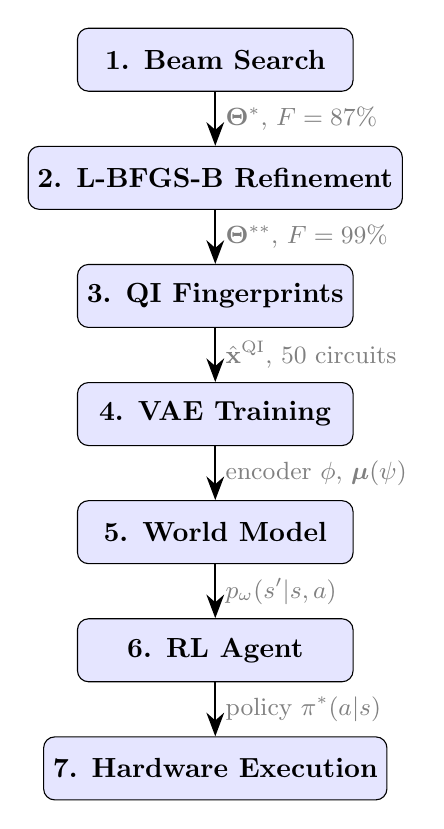
\begin{tikzpicture}[
    box/.style={rectangle, draw, rounded corners, minimum width=3.5cm, minimum height=0.8cm,
                text centered, fill=blue!10},
    arrow/.style={-{Stealth[length=3mm]}, thick},
    note/.style={text=gray, font=\small}
]
\node[box] (bs)  at (0,0)    {\textbf{1. Beam Search}};
\node[box] (ref) at (0,-1.5) {\textbf{2. L-BFGS-B Refinement}};
\node[box] (qi)  at (0,-3.0) {\textbf{3. QI Fingerprints}};
\node[box] (vae) at (0,-4.5) {\textbf{4. VAE Training}};
\node[box] (wm)  at (0,-6.0) {\textbf{5. World Model}};
\node[box] (rl)  at (0,-7.5) {\textbf{6. RL Agent}};
\node[box] (hw)  at (0,-9.0) {\textbf{7. Hardware Execution}};

\draw[arrow] (bs)  -- (ref) node[midway, right, note] {$\boldsymbol{\Theta}^*$, $F=87\%$};
\draw[arrow] (ref) -- (qi)  node[midway, right, note] {$\boldsymbol{\Theta}^{**}$, $F=99\%$};
\draw[arrow] (qi)  -- (vae) node[midway, right, note] {$\hat{\mathbf{x}}^{\mathrm{QI}}$, 50 circuits};
\draw[arrow] (vae) -- (wm)  node[midway, right, note] {encoder $\phi$, $\boldsymbol{\mu}(\psi)$};
\draw[arrow] (wm)  -- (rl)  node[midway, right, note] {$p_\omega(s'|s,a)$};
\draw[arrow] (rl)  -- (hw)  node[midway, right, note] {policy $\pi^*(a|s)$};
\end{tikzpicture}
\end{center}

\medskip

\begin{table}[h]
\centering
\begin{tabular}{llll}
\toprule
\textbf{Step} & \textbf{Input} & \textbf{Output} & \textbf{Cost} \\
\midrule
1. Beam Search    & Ansatz, $\Delta_s$         & Top trajectories $\boldsymbol{\Theta}^*$ & Cheap (sim) \\
2. Refinement     & $\boldsymbol{\Theta}^*$    & $\boldsymbol{\Theta}^{**}$, $F\geq99\%$ & Cheap (sim) \\
3. QI Acquisition & $\boldsymbol{\Theta}^{**}$ & $\{\hat{\mathbf{x}}_j^{\mathrm{QI}}\}$  & 50 QI runs  \\
4. VAE            & $\hat{\mathbf{x}}$         & Latent $\boldsymbol{\mu}$, encoder $\phi$ & GPU hours  \\
5. World Model    & $(\boldsymbol{\mu}_t, \mathbf{a}_t, \boldsymbol{\mu}_{t+1})$ & $f_\omega, \boldsymbol{\sigma}_\omega$ & GPU hours \\
6. RL             & $f_\omega$                 & Policy $\pi^*$                           & GPU hours  \\
7. Hardware       & $\pi^*$                    & GHZ state, $F_{\mathrm{hw}}$             & QI runs    \\
\bottomrule
\end{tabular}
\caption{Pipeline summary. QI = Quantum Inspire hardware runs.}
\end{table}

\end{document}
